% !TEX program = pdflatex
% Two-column résumé — uses paracol so columns can break across pages (fixes huge blank gaps).
% Compile: pdflatex resume.tex

\documentclass[a4paper,10pt]{article}

\usepackage[T1]{fontenc}
\usepackage[utf8]{inputenc}
\usepackage[default]{sourcesanspro}
\usepackage{microtype}
\usepackage[a4paper,top=16mm,bottom=16mm,left=16mm,right=16mm]{geometry}
\usepackage{xcolor}
\usepackage{ragged2e}
\usepackage{tikz}
\usetikzlibrary{calc}
\usepackage{paracol}
\usepackage[hidelinks]{hyperref}

\IfFileExists{fontawesome5.sty}{%
  \usepackage{fontawesome5}%
  \newcommand{\IconLoc}{\textcolor{textgray}{\small\faMapMarker*}\;}
  \newcommand{\IconMail}{\textcolor{textgray}{\small\faEnvelope}\;}
  \newcommand{\IconPhone}{\textcolor{textgray}{\small\faPhone*}\;}
  \newcommand{\IconWeb}{\textcolor{textgray}{\small\faGithub}\;}
  \newcommand{\IconLi}{\textcolor{textgray}{\small\faLinkedin}\;}
}{%
  \newcommand{\IconLoc}{\textcolor{textgray}{$\triangleright$\;}}
  \newcommand{\IconMail}{\textcolor{textgray}{$\triangleright$\;}}
  \newcommand{\IconPhone}{\textcolor{textgray}{$\triangleright$\;}}
  \newcommand{\IconWeb}{\textcolor{textgray}{$\triangleright$\;}}
  \newcommand{\IconLi}{\textcolor{textgray}{$\triangleright$\;}}
}

\definecolor{textblack}{HTML}{151515}
\definecolor{textgray}{HTML}{6B6B6B}
\definecolor{hairline}{HTML}{D0D0D0}

\hypersetup{colorlinks=true, linkcolor=textblack, urlcolor=textgray}

\setlength{\parindent}{0pt}
\setlength{\parskip}{0pt}
\pagestyle{empty}
\raggedbottom

\newcommand{\sidebarheading}[1]{%
  \vspace{0.55em}%
  {\bfseries\fontsize{6.8}{8}\selectfont\textls[200]{\MakeUppercase{#1}}\par}%
}

\newcommand{\sidebarsub}[1]{%
  \vspace{0.35em}%
  {\bfseries\fontsize{6.5}{7.8}\selectfont\textls[140]{\MakeUppercase{#1}}\par}%
  \vspace{0.25em}%
}

\newcommand{\mainheading}[1]{%
  \vspace{0.35em}%
  {\bfseries\fontsize{6.8}{8}\selectfont\textls[160]{\MakeUppercase{#1}}\par}%
  \vspace{0.45em}%
}

\newcommand{\hollowbullet}{\textcolor{textgray}{\fontsize{11}{11}\selectfont$\circ$\kern1pt}}

\newcommand{\jobtitlebar}[2]{%
  {\bfseries\fontsize{8.4}{10}\selectfont\textls[70]{\MakeUppercase{#1}}\ %
  \textcolor{textgray}{\fontsize{8.4}{10}\selectfont\textls[70]{\textbar}}\ %
  {\bfseries\fontsize{8.4}{10}\selectfont\textls[70]{\MakeUppercase{#2}}}\par}%
}

\newcommand{\firmline}[1]{%
  \vspace{0.2em}%
  {\bfseries\fontsize{7.8}{9.2}\selectfont\textls[55]{\MakeUppercase{#1}}\par}%
}

\newcommand{\stackline}[1]{%
  \vspace{0.22em}%
  {\color{textgray}\fontsize{7.6}{9.8}\selectfont\textbf{Stack:} #1\par}%
}

\newcommand{\exbullet}{\raisebox{0.12ex}{\textcolor{textblack}{\rule{3.2pt}{3.2pt}}}\kern5pt}

% One job = circle + text (no page-trapping mega-tikz). Optional connector stub downward.
\newcommand{\jobentry}[2]{%
  \par\vspace{0.75em}%
  \noindent
  \begin{minipage}[t]{6mm}%
    \centering\vspace{0pt}%
    
\begin{tikzpicture}[baseline=-0.55ex]
      \draw[fill=white,draw=hairline,line width=0.65pt] (0,0) circle (3.6pt);
    \end{tikzpicture}%
  \end{minipage}%
  \hspace{3pt}%
  \begin{minipage}[t]{\dimexpr\linewidth-9mm}%
    #1%
    #2%
  \end{minipage}%
}

\begin{document}
\color{textblack}
\fontsize{9.5}{12.4}\selectfont

% ----- Header (full width) -----
\noindent
\begin{minipage}[t]{0.68\textwidth}
\raggedright
{\fontsize{9}{11}\selectfont\fontseries{m}\selectfont\textls[220]{\MakeUppercase{Mattias}}\par}
\vspace{-5pt}
{\fontsize{36}{38}\selectfont\bfseries\textls[45]{\MakeUppercase{Gebrie}}\par}
\vspace{9pt}
{\color{textgray}\fontsize{8.3}{10}\selectfont\fontseries{l}\selectfont\textls[220]{\MakeUppercase{Data Science Student \& Full Stack Developer}}\par}
\end{minipage}\hfill
\begin{minipage}[t]{0.22\textwidth}\raggedleft
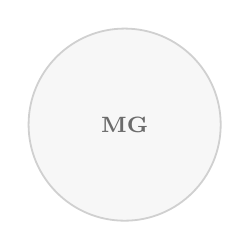
\begin{tikzpicture}
  \draw[hairline,line width=0.65pt,fill=black!3] (0,0) circle (1.22cm);
  \node[font=\footnotesize\bfseries\color{textgray}] at (0,0) {MG};
\end{tikzpicture}
\end{minipage}

\vspace{10pt}

\noindent{\color{hairline}\rule{0.65pt}{11mm}\hspace{3mm}}

\vspace{6pt}

% ----- Body: paracol allows breaks; NEVER use \rule{\textheight} inline (destroys layout) -----
\columnratio{0.31,0.69}
\setlength{\columnsep}{7mm}
\begin{paracol}{2}

\sidebarheading{Contact}

\vspace{0.35em}
{\fontsize{8}{11}\selectfont\color{textgray}
\IconLoc\textbf{Location}\par\vspace{1pt}\hspace{1.15em}Norway\par\vspace{0.45em}
\IconMail\textbf{Email}\par\vspace{1pt}\hspace{1.15em}Available upon request\par\vspace{0.45em}
\IconPhone\textbf{Phone}\par\vspace{1pt}\hspace{1.15em}Available upon request\par\vspace{0.45em}
\IconWeb\textbf{GitHub}\par\vspace{1pt}\hspace{1.15em}\href{https://github.com/atomattias}{github.com/atomattias}\par\vspace{0.45em}
\IconLi\textbf{LinkedIn}\par\vspace{1pt}\hspace{1.15em}\href{https://www.linkedin.com/in/gmattias/}{linkedin.com/in/gmattias}\par}

\vspace{10pt}

\sidebarheading{Skills}

\sidebarsub{Professional}
\hollowbullet Cross-functional collaboration\par\vspace{0.12em}
\hollowbullet Technical writing \& documentation\par\vspace{0.12em}
\hollowbullet Stakeholder communication\par\vspace{0.12em}
\hollowbullet Agile / iterative delivery\par

\vspace{0.45em}

\sidebarsub{Technical}
\hollowbullet C\#, Java, Python, C++, Spring Boot\par\vspace{0.12em}
\hollowbullet React, React Native, Next.js, JavaScript\par\vspace{0.12em}
\hollowbullet AWS, Azure, Docker, Kubernetes\par\vspace{0.12em}
\hollowbullet Apache Spark, Git, TensorFlow\par

\vspace{10pt}

\sidebarheading{Education}

\vspace{0.35em}
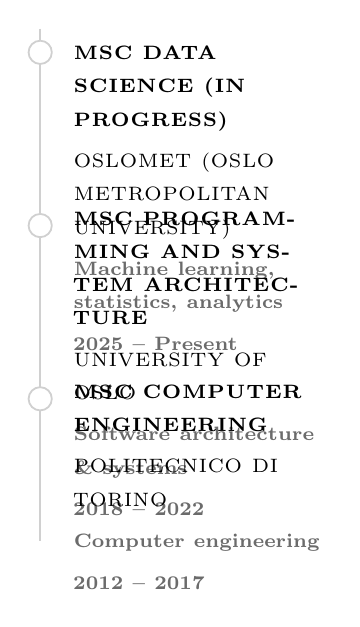
\begin{tikzpicture}[x=1mm,y=1mm]
  \def\rail{3.8}
  \def\h{62}
  \draw[hairline,line width=0.75pt] (\rail,3) -- (\rail,-\h);
  \foreach \y in {0,-22,-44}{
    \draw[fill=white,draw=hairline,line width=0.65pt] (\rail,\y) circle (4.2pt);
  }
  \node[anchor=north west, align=left, text width=0.26\columnwidth] at (\rail+5.5mm,2mm) {%
    {\bfseries\fontsize{7}{8.4}\selectfont\textls[40]{\MakeUppercase{MSc Data Science (in progress)}}}\par\vspace{3pt}%
    {\fontsize{7}{8.4}\selectfont\textls[35]{\MakeUppercase{OsloMet (Oslo Metropolitan University)}}}\par\vspace{3pt}%
    \textcolor{textgray}{\fontsize{6.9}{8}\selectfont\bfseries Machine learning, statistics, analytics}\par\vspace{3pt}%
    \textcolor{textgray}{\fontsize{7}{8}\selectfont\bfseries 2025 -- Present}};

  \node[anchor=north west, align=left, text width=0.26\columnwidth] at (\rail+5.5mm,-19mm) {%
    {\bfseries\fontsize{7}{8.4}\selectfont\textls[40]{\MakeUppercase{MSc Programming and System Architecture}}}\par\vspace{3pt}%
    {\fontsize{7}{8.4}\selectfont\textls[35]{\MakeUppercase{University of Oslo}}}\par\vspace{3pt}%
    \textcolor{textgray}{\fontsize{6.9}{8}\selectfont\bfseries Software architecture \& systems}\par\vspace{3pt}%
    \textcolor{textgray}{\fontsize{7}{8}\selectfont\bfseries 2018 -- 2022}};

  \node[anchor=north west, align=left, text width=0.26\columnwidth] at (\rail+5.5mm,-41mm) {%
    {\bfseries\fontsize{7}{8.4}\selectfont\textls[40]{\MakeUppercase{MSc Computer Engineering}}}\par\vspace{3pt}%
    {\fontsize{7}{8.4}\selectfont\textls[35]{\MakeUppercase{Politecnico di Torino}}}\par\vspace{3pt}%
    \textcolor{textgray}{\fontsize{6.9}{8}\selectfont\bfseries Computer engineering}\par\vspace{3pt}%
    \textcolor{textgray}{\fontsize{7}{8}\selectfont\bfseries 2012 -- 2017}};
\end{tikzpicture}

\switchcolumn

\mainheading{Profile}
{\justifying\fontsize{8.9}{12}\selectfont
Currently pursuing a Master's in Data Science at OsloMet, building upon a strong academic foundation with two completed master's degrees in Computer Engineering and System Architecture. With over 10 years of hands-on experience in system development and data engineering, I'm now specializing in AI/ML techniques and data science methodologies. Expertise in backend development (C\#, Java, Python, C++), cloud technology (AWS, Azure), and big data processing (Apache Spark). Published researcher with hands-on experience in machine learning, TensorFlow, and IoT security. Passionate about applying advanced analytics to solve real-world problems and extract meaningful insights from complex datasets.\par}

\vspace{8pt}

\mainheading{Experience}

\jobentry{%
  \jobtitlebar{Teaching Assistant}{Feb 2026 -- May 2026}%
  \firmline{OsloMet (Oslo Metropolitan University)}%
}{%
  \vspace{0.28em}\fontsize{8.4}{11}\selectfont
  \exbullet ACIT4830 --- Machine Learning for Robotics and Automation\par\vspace{0.12em}%
  \exbullet ACIT4290 --- Practical Cyber Security\par
}

\jobentry{%
  \jobtitlebar{Application Support Specialist}{Feb 2025 -- Jun 2025}%
  \firmline{C-Loop}%
}{%
  \vspace{0.28em}\fontsize{8.4}{11}\selectfont
  ERP testing and technical support for enterprise applications.\par
}

\jobentry{%
  \jobtitlebar{User Support Technician}{Sep 2022 -- Feb 2025}%
  \firmline{Itec International Arora}%
}{%
  \vspace{0.28em}\fontsize{8.4}{11}\selectfont
  Technical user support and troubleshooting.\par
}

\jobentry{%
  \jobtitlebar{Freelance Developer}{Jul 2021 -- Present}%
  \firmline{Self-employed}%
}{%
  \vspace{0.28em}\fontsize{8.4}{11}\selectfont
  Built a cross-platform mobile application; owned delivery end-to-end with emphasis on usability and UX. Partnered with designers to ship features that improved satisfaction.\par
  \stackline{Spring Boot, React Native, Next.js}%
}

\jobentry{%
  \jobtitlebar{Web Developer}{Aug 2022 -- Dec 2022}%
  \firmline{School of Applied Technology (SALT)}%
}{%
  \vspace{0.28em}\fontsize{8.4}{11}\selectfont
  Mobile application development with React Native and .NET.\par
}

\jobentry{%
  \jobtitlebar{Data Engineer}{Jun 2021 -- Aug 2021}%
  \firmline{Schibsted Data Foundation}%
}{%
  \vspace{0.28em}\fontsize{8.4}{11}\selectfont
  Built and operated ETL-oriented data pipelines.\par
  \stackline{AWS, React Library, Java, Scala, Git, Jenkins, Travis, Spinnaker}%
}

\jobentry{%
  \jobtitlebar{Backend Developer}{Jul 2019 -- Sep 2019}%
  \firmline{Simula}%
}{%
  \vspace{0.28em}\fontsize{8.4}{11}\selectfont
  Improved mobile broadband reliability via multi-connection approaches; developed TensorFlow-based algorithms for network performance.\par
  \stackline{Python, TensorFlow}%
}

\jobentry{%
  \jobtitlebar{System Developer}{Nov 2007 -- Sep 2012}%
  \firmline{Jimma University}%
}{%
  \vspace{0.28em}\fontsize{8.4}{11}\selectfont
  Delivered open-source IP telephony, mail server, and Active Directory infrastructure.\par
}

\vspace{9pt}

\mainheading{Publications}
{\justifying\fontsize{8.4}{11.2}\selectfont
\textbf{M. T. Gebrie and H. Abie,} ``Risk-based adaptive authentication for internet of things in smart home eHealth,'' in \textit{Proceedings of the 11th European Conference on Software Architecture: Companion Proceedings,} 2017, pp.\ 102--108. ACM.\par}

\end{paracol}

\end{document}
